\begin{figure}[t!]
	\centering
  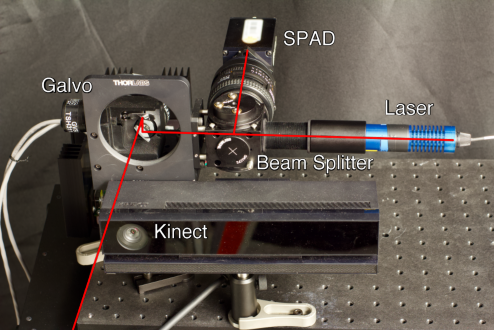
\includegraphics[width=0.8\columnwidth]{prototype_single_col.pdf}
  \caption{Prototype scanning setup. The pulsed light from the laser travels
    through a beam splitter before being guided by the galvo to the scene.
    Returning light is measured by the single-pixel SPAD. The RGB camera of a
    Kinect v2 is used to capture the monocular RGB image (the depth camera is
    not used)}
  \label{fig:prototype}
\end{figure}

%%%%%%%%%%%%%%%%%%%%%%%%%%%%%%%%%%%%%%%%%%%%%%%%%%%%%%%%%%%%%%%%
\subsection{Prototype RGB-SPAD Camera Hardware}

% The laser operates at 450~nm with a pulse repetition rate of 25~MHz with a peak power of 450~mW and average power of 0.5~mW.

As shown in Figure~\ref{fig:prototype}, our prototype camera comprises a color camera (Microsoft Kinect v2), a single-pixel SPAD (Micro Photon Devices 100~$\mu m$ PDM series, free-running), a laser (ALPHALAS PICOPOWER-LD-450-50), and a two-axis galvanometer mirror system (Thorlabs GVS012). The laser operates at 670~nm with a pulse repetition rate of 10~MHz with a peak power of 450~mW and average power of 0.5~mW. The SPAD records temporal histograms with 16384 bins, each corresponding to a time window of 16~ps. SPAD and laser are co-axially aligned using a beam splitter (Thorlabs PBS251). The full width at half maximum (FWHM) of the combined laser pulse width and SPAD jitter is about 70~ps, allowing the system to record depth map with an accuracy of about 1~cm. A National Instruments data acquisition device (NI-DAQ USB-6343) provides synchronization signals for the galvos, SPAD, and laser. The ground truth depth map is raster-scanned at a resolution of $512 \times 512$ pixels. The single-pixel, diffused SPAD measurement is generated by summing all of these measurements for a specific scene. This allows us to validate the accuracy of the proposed histogram matching algorithm that only uses the single histogram of the diffused SPAD and compare it with ground truth. Monocular depth estimation is calculated using the RGB image captured by the Kinect v2.

%We determined camera intrinsics and extrinsics for the Kinect's RGB camera and
%the scanning system using the standard camera calibration toolbox in MATLAB.
%In general it is impossible to compensate for the offset between camera and
%SPAD, but we do add the z displacement from spad to kinect to partially
%compensate for it.
%% \textcolor{red}{Mark, please write a short paragraph on calibration details, including any warping of the SPAD histograms you did to compensate for the offset in camera and SPAD position.}
%
%Missing:
%%
%\begin{itemize}
%\item RGB resolution used for MDE
%\item do we also have Kinect depth maps for comparison? (yes) kinect resolution: RGB is 1920x1080 and depth camera is 512x424
%\end{itemize}

%%%%%%%%%%%%%%%%%%%%%%%%%%%%%%%%%%%%%%%%%%%%%%%%%%%%%%%%%%%%%%%%
\subsection{Experimental Results}

Using this prototype, we captured a number of scenes as shown in
Figure~\ref{fig:results_captured} and in the supplement. We crop the RGB image
to have dimensions that are multiples of 32. For DORN only, we further
downsample the image to a resolution of $353 \times 257$. We then feed this RGB
image into the monocular depth estimation algorithm. In Figure~\ref{fig:results_captured} we show a subset of the scenes we captured and processed with MiDAS~\cite{Lasinger:2019}, which achieved the best results among the depth estimators we tested. Additional scenes, also processed with other MDE approaches, including DenseDepth~\cite{Alhashim2018} and DORN~\cite{Fu2018}, are included in the supplement. The ground truth depth is captured with the scanned SPAD, as described above, and regions with low signal-to-noise ratio are masked out (shown in black).

In the first two examples, the ``Hallway'' and ``Conference Room'' scenes, we see that the monocular depth CNN estimates the ordinal depth of the scene reasonable well. However, the root mean squared error (RMSE) for these two scenes is relatively high with 2.4--2.9~m (see red/white error maps in Fig.~\ref{fig:results_captured}). The proposed method using a single diffused SPAD measurement corrects this systematic depth estimation error and brings the RMSE down to 0.6--0.9~m. The ``Poster'' scene is meant to confuse the CNN---it shows a flat poster with a printed scene. As expected, the CNN predicts that the statue is closer than the arches in the background, which is incorrect in this case. The proposed method uses the SPAD histogram to correctly flatten the estimated depth map. 

\begin{figure}[t]
	\centering
	\includegraphics[width=\columnwidth]{captured_results_main}
	\caption{Experimental results. For each scene, we record an RGB image (lower left subimages) and a ground truth depth map that is raster-scanned with the SPAD (upper left subimages). A monocular depth CNN often predicts the ordinal depth well (top two scenes), which is corrected with the diffused SPAD histogram using the proposed method (top right subimages) as shown by the error maps and root mean squared error (RMSE) for each example (lower center and right subimages). The CNN is confused when we show it a photograph of a poster (bottom scene); it incorrectly predicts the depth of the scene depicted on the flat print. Our method is able to correct this error. }
	\label{fig:results_captured}
\end{figure}
